\section{Results}\label{sec:results}
\subsection{Pilot trend-recovery RMSE}
Table~\ref{tab:rmse} and Figure~\ref{fig:rmse} summarize the descriptive means over pilot design cells. Under fixed $\mu=0$, profiled marginal ML has the smallest average of these implementations. The 20-seed pilot is too narrow to establish a universal criterion ranking or statistical significance, and mean policies use paired observations. The original BIC positive-grid result is strongly affected by its first admissible $s$ candidate.

\begin{table*}[t]
\caption{Pilot average RMSE against known latent-trend truth; only difference orders 1--6. Residual BIC here uses the original S grid, whose smallest positive point is 0.01, not an unrestricted optimum.}
\label{tab:rmse}\centering
\begin{tabular}{lrr}
\toprule
Selection criterion & Fixed $\mu=0$ & Plug-in $\widehat\mu=\overline{D_dy}$\\
\midrule
CV & 0.174451 & 0.193489\\
GCV & 0.176647 & 0.194667\\
AICc & 0.157946 & 0.177608\\
RSS-based BIC (positive grid) & 0.297390 & 0.297390\\
Profiled Gaussian marginal ML & 0.140633 & 0.178623\\
\bottomrule
\end{tabular}
\end{table*}

\begin{figure}[t]\centering
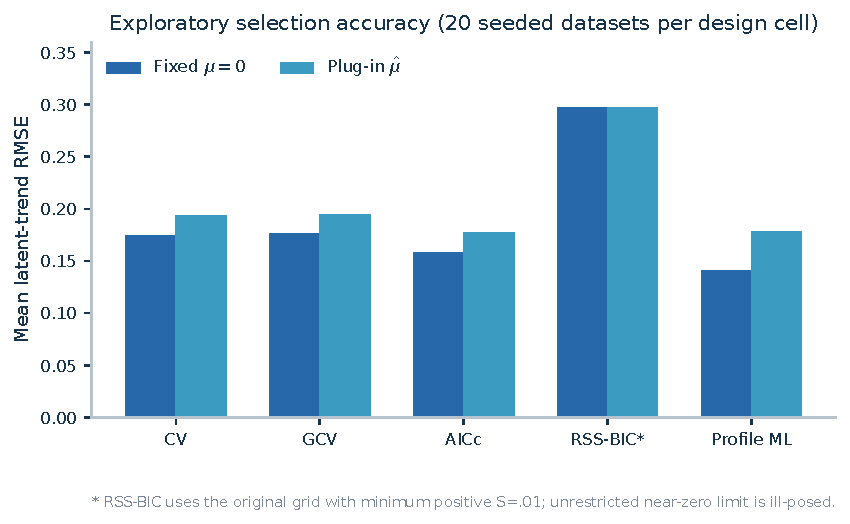
\includegraphics[width=\columnwidth]{figures/rmse_criteria.pdf}
\caption{Mean true-trend recovery RMSE across the exploratory pilot configurations. Lower values indicate better recovery under the particular generating mechanism. BIC's near-interpolation behavior makes its original grid selection nonrepresentative of an unrestricted optimum; comparisons are descriptive, not inferential rankings.}
\label{fig:rmse}
\end{figure}

\subsection{Numerical stability against 85-digit fitted trends}
The independent high-precision calculation establishes which floating-point methods actually solve the same specified PLS problem reliably in the tested extreme-$s$ regimes. Table~\ref{tab:precision} and Figure~\ref{fig:precision} summarize 576 attempts per implementation. The shift-free full SVD yields maximum observed relative error $5.52\times10^{-9}$ without failed fits or errors above $10^{-5}$. Scaled augmented QR offers an independent comparison with maximum $3.10\times10^{-9}$. Ordinary primal double-precision banded Cholesky fails on 216 cases and returns relative errors above $10^{-5}$ in 294 of its 360 completed cases.

\begin{table*}[t]
\caption{Numerical comparisons with the independent 85-digit reference, condensed into four paired rows. Every method was attempted on 576 matched problems. The Large/fail column counts completed fits with relative error above $10^{-5}$ and factorization failures, respectively. Results for the additional minimum-norm SVD method remain in the raw archive.}
\label{tab:precision}\centering
\setlength{\tabcolsep}{4pt}
\begin{tabular}{@{}lrr@{\qquad}lrr@{}}
\toprule
Method & Max.\ error & Large/fail &
Method & Max.\ error & Large/fail\\
\midrule
Shift-free SVD & $5.52\,10^{-9}$ & 0/0 &
Scaled QR & $3.10\,10^{-9}$ & 0/0\\
Polynomial-ref.\ SVD & $3.85\,10^{-6}$ & 0/0 &
Dual SVD & $3.69\,10^{-8}$ & 0/0\\
Stacked SVD & $1.57\,10^{-5}$ & 12/0 &
Dual banded Cholesky & $1.22\,10^{-1}$ & 302/0\\
Primal banded Cholesky & $6.81\,10^{2}$ & 294/216 &
Gram eigendecomp.\ & $1.45\,10^{2}$ & 484/0\\
\bottomrule
\end{tabular}
\end{table*}

\begin{figure*}[t]\centering
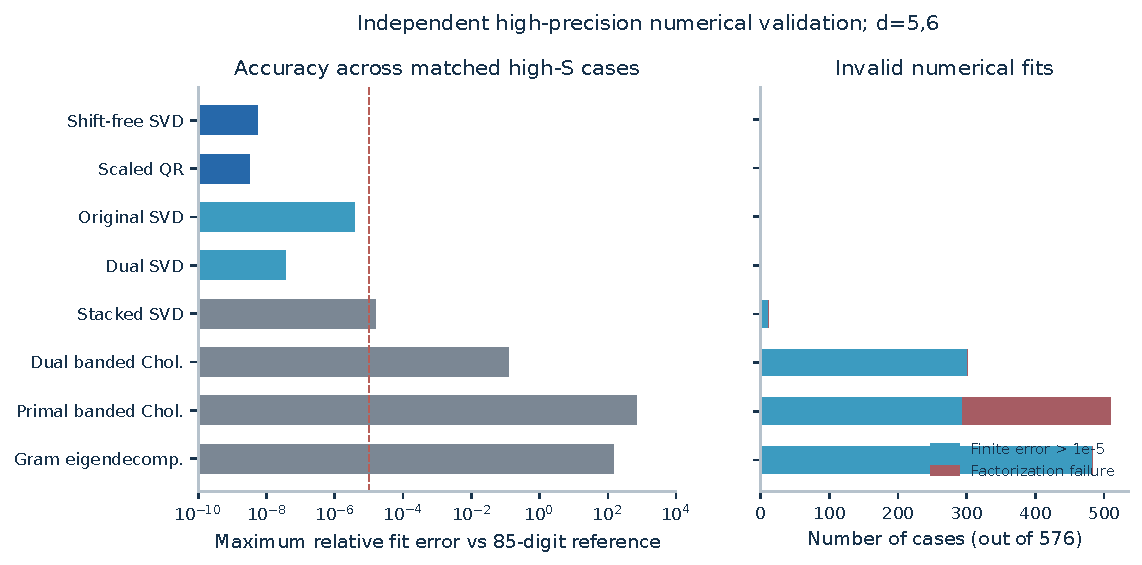
\includegraphics[width=\textwidth]{figures/solver_accuracy.pdf}
\caption{High-smoothness numerical validation in four paired rows, with two methods per row. Left: maximum relative fit error against the 85-digit reference; right: finite errors above $10^{-5}$ and factorization failures.}
\label{fig:precision}
\end{figure*}

This numerical evidence motivates **full SVD of $D_d$ with shift-free reconstruction as the default for this spectral framework**. The scaled QR result is important corroboration, and the conclusion is about validity and accuracy on the tested configurations rather than execution speed. In particular the structure-exploiting Cholesky algorithms of earlier work remain relevant for other conditioning regimes and for performance-sensitive workloads \citep{weinert2007,biessy2026}.

\subsection{Restricted residual-BIC sensitivity}
Applying the unchanged published BIC score on $s\ge0.05$ gives average true-trend RMSE 0.290446, and all 1,920 selections attain the imposed lower limit. Restricting to $s\ge0.10$ gives mean RMSE 0.245280, with 1,535 of 1,920 selections at its lower limit. This is a sensitivity result, not a resolution of the mathematical divergence.

\begin{figure*}[t]\centering
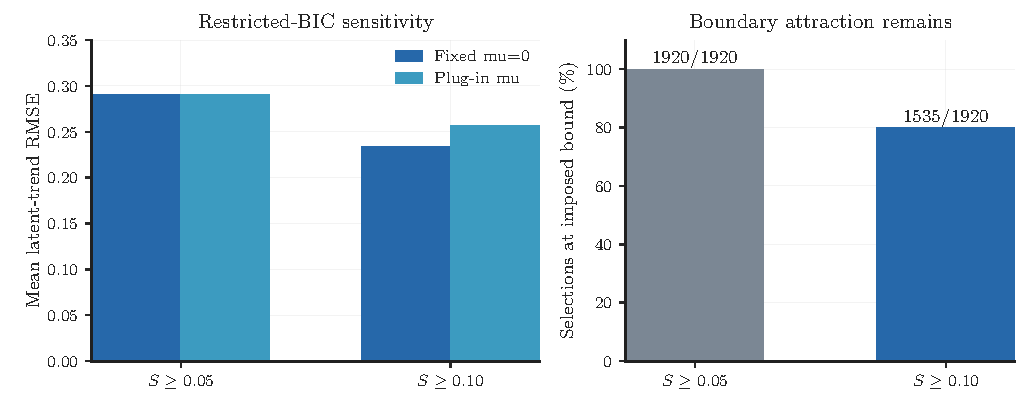
\includegraphics[width=\textwidth]{figures/restricted_bic.pdf}
\caption{Restricted residual-BIC sensitivity on the same pilot observations. Left: mean recovery RMSE by reference-mean policy. Right: percentage of searches selecting the explicitly imposed minimum $s$. Counts use 1,920 correlated criterion/order/mean rows per restriction, not independent experiments.}
\label{fig:restricted}
\end{figure*}
